\documentclass[referee]{aa}
\usepackage{graphicx}
\usepackage[numbers]{natbib}
\usepackage{txfonts}

\begin{document}
%
   \title{Notes on photo-z for the LSST}

   \author{J. Cohen-Tanugi, E. Giraud, E. Nuss
          }



   \institute{Laboratoire Univers et Particules de Montpellier,
              UMR5299 CNRS-In2p3/Montpellier University, F-34095 Montpellier
             }

   
   \date{}
\authorrunning{J. Cohen-Tanugi, E. Giraud, E. Nuss}
\titlerunning{Note on photo-z}

\abstract{Deriving redshifts without spectroscopy is a major challenge for the LSST. We have embarked in the preparation of a dedicated photo-z tool.}
 {Our first step is to 
build a set of template spectra and spectral sequences around them. We use a spectroscopic pilot survey in the range $0.3 \leq z \leq 1$, that is reasonably complete up to $R = 23$.}
{The spectra are first divided in 4 classes, depending on their blue or red SED, absorption or emission lines, and 5 redshift bins from $z = 0.3$ to $z = 1$, measured in the rest frame window 
3000 \AA ~- 6000 \AA.  The stellar mixing and synthetic spectra are derived from the SED using the $\it starlight$ code in that wavelength range, then the model continuum spectra are extended to the range 1000 \AA ~- 10 000 \AA.}
{The 4000 \AA~break is the main feature in all spectra at all redshifts considered.  
There are two distinct classes of
spectra depending on their general shape above 3000  \AA . The first one includes early absorption systems,  most
of the post-starbursts, red spirals at $z \leq 0.6-0.7$, the second one includes blue star-forming galaxies and recent
post-starbursts. Among galaxies of the first class the 4300 \AA~ step declines with $z$ around
$z = 0.6-0.7$ in red spirals, and around $z = 1$ in early ellipticals. All spectra with some recent stellar activity show a clear UV excess between 1500 \AA~ and 2500 \AA.
Large variations in the UV  due to a residual fraction of young stars in early absorption
systems or to the age and intensity of the most recent starburst in post-starburst galaxies,
may occurr at any look back time. Red emission lines galaxies show an increasing fraction of young stars with $z$ and a decreasing
fraction of stars older than $\rm \leq 2.5~ Gyr$. } 
{The next step is to compare with a spectroscopic atlas. Then we will derive photometric SED, and test our template sequences on photometric surveys with redshifts.}

\keywords{cosmology  - spectral energy distribution - evolution}
           

 \maketitle
 

%______________________________________________________________

\section{Introduction}


In the course of an investigation of the diffuse intergalactic light we obtained
galaxy redshifts and spectral flux distributions in a pencil beam of 10' x 10' at magnitude brighter than R = 23
\citep{Catalog:2012}. Redshift completeness is shown in Figure~\ref{central_R}.
This pencil beam survey covers  a redshift range up to z = 1 (with some galaxies up to z = 1.7). It compares in size 
with the DEEP1 spectroscopic pilot survey \citep{Weiner:2005}. 
In standard cosmology with $H_o = 75$~$\rm km~s^{-1}~Mpc^{-1}$, $\Omega_{0,m}=0.30$, and $\Omega_{0,\Lambda} = 0.70$,
this range provides a large leverage of about 3000~Mpc or 7~Gyr. Our sample
was indeed sufficient to extract
some of the most conspicuous characteristics on galaxy evolution at $z \leq 1$ (see below).

We will use our pilot survey to prepare a library of spectra covering
the main characteristics of galaxy spectra up to z = 1. About half
of all stars seem to be still forming, mostly in disks, in this range \citep{Dickinson:2003p4993, Hammer:2005p5042}.

Galaxy colors have been shown to segregate in a bimodal distribution 
\citep{Strateva:2001p5121, Hogg:2002p5043, Blanton:2003p4432} even for field 
galaxies, corresponding respectively to E, S0, Sa, and Sb, Sc, Irr in the 
Sloan Digital Sky Survey \citep[SDSS,][]{York:2000p5225}. The extensive work on the 
Cosmic Evolution Survey \citep[COSMOS,][]{Scoville:2007p5137}, 
confirmed this double distribution between a ``red sequence'' and a 
``blue cloud''  up to $z = 0.7$  \citep[][ and references therein]{Cassata:2007p4503}, 
a behavior that seems to hold at even higher redshifts
\citep[$z \sim 1$,][]{Bell:2004p4427}; and up to $z \sim 1.5-2$
\citep{Giallongo:2005p5002, Cucciati:2006p4973, Franzetti:2007p4273}. 
Studies based upon extensive data sets \citep{LeFevre:2007p5105, Franzetti:2007p4273}
have shown that the relative weight of red and blue objects in the bimodal distribution changes 
with $z$ and environment \citep{LeFevre:2007p5105, Franzetti:2007p4273}. More precisely,
an increase of massive red galaxies with cosmological time was discovered
\citep[][ DEEP2 and COMBO-17 data]{Bell:2004p4427, Faber:2007}. 

More than a decade ago, \cite{Cowie:1996p4930} suggested that
while the most massive galaxies were formed early
in the Universe, star formation is progressively shifted to smaller systems,
the so-called downsizing effect. This effect had been confirmed
by several later studies \citep{Kodama:2004p5056, Bell:2005p4431}.
This downsizing detected in samples of galaxies at different redshifts has been termed ``downsizing in time''
to be distinguished from the ``archaeological downsizing'' which refers to the observation that less massive early 
type galaxies formed their stellar populations later and over a longer time span
than the more massive ones \citep{Thomas:2005p5302, Clemens:2006p5321}.

Several studies suggest that the bulk of 
stars in  early-type cluster galaxies had a formation redshift of $z \geq 3$, 
while those in lower density environments may have formed later, but still at 
$z \geq 1.5-2$ \citep[for reviews see][]{Renzini:2006p5117, Renzini:2007p5120}. 
This may be in contradiction with the rise in the number of massive red galaxies
found by Faber et al. (2007) who concluded that most early types galaxies reached
their final form below $z =1$. Our data include a clear red sequence at  $z = 0.29$ 
and a quite large number of absorption systems up to $z \sim 1$ which we fit
with population synthesis models in order to search for age variations with
$z$ and luminosity.

The main known features of galaxy evolution visible in the
pencil beam survey are listed below:
\begin{enumerate}

\item Elliptical galaxies. Absorption-line galaxies do not show significant variation in their continuum energy distributions up to $z = 0.6$ and a moderate decrease of the 4000~\AA\  break amplitude of $6\%$ at $z \sim 0.82$, and $15\%$ at $z \sim 1$.  
Galaxies at $z \geq 0.8$ still had some star formation about 1 Gyr earlier. 

\item Archeological downsizing. The faint absorption-line galaxies in our dynamically young cluster at  
$z = 0.29$ have indexes similar to those of bright absorption-line systems at $z = 0.8$, suggesting that faint galaxies without emission lines tend 
to be younger than  more massive galaxies with similar spectra.  Our population synthesis models indicate that $\rm 50 \%$ of the stars contributing 
to the spectra of faint absorption-line galaxies at z = 0.29 were formed at $z < 1$. This is consistent with cases of truncated red sequences observed in some 
high-$z$ clusters and suggests that clusters with truncated red-sequences may be dynamically young. This also suggests that the red sequence
is still in a building phase at $z \leq 1$.

\item The average spectra of galaxies with emission lines show significant systematic variations in their energy distribution 
with $z$, consistent with what is observed in other regions of the Universe. 

\item Downsizing of starbursts. The intrinsic luminosities of starbursts decline with cosmological time,
and continue to decrease also in the next evolutionary phase. Therefore, downsizing
must take place  both in luminosity {\it and} in number density. In our sample the ``down-sizing'' phenomenon is of $1.2-1.7$ magnitudes from $z = 0.4$ to $z = 0.9$

\item When we divide the sample of emission-line galaxies in two halves by continuum color, we find that the spectral variations are consistent with the following scenario: 

\begin{enumerate} 
   \item the brightest red emission-line galaxies at $z < 0.5$ have the oldest stellar populations; 
   \item the Universe at $z \leq 0.65$ is repopulated with starburst galaxies at a constant rate down
	to $z\simeq0.3$ while at $z \geq 0.65$ the birthrate of starbursts, or the AGN fraction, is higher;
   \item the red half of emission-line galaxies become redder with decreasing redshift and have lower EQW([OII]) and higher D(4000).
\end{enumerate}

\item The red limit in the energy distribution of emission-line galaxies at $z \leq 0.6$ is typical of bulge-dominated spiral galaxies with moderate 
star formation, and of early-type LINERs.

\end{enumerate}

The Note is structured as follows. Section~2 describes the survey properties and the method of analysis. The next sections focus on absorption systems, post starbursts,
emission lines galaxies with blue and red continuum. Preliminary conclusions are in Section~\ref{conclusion}.

%SECTION 2

\section{Observations, data reduction and survey properties}

The observations (ESO program 078A-0456(A) were obtained with the FORS2 instrument \citep{fors:2005} on the Cassegrain focus
of the VLT UT1 telescope in multi-object spectroscopy mode with the exchangeable mask unit (MXU).
 The data reduction, quality of the spectra, and analysis  \citep{Giraud:2011} are not repeated here. Figure~\ref{central_R} shows 
 the $R$-magnitude histogram of the galaxies with measured redshifts
superimposed on the magnitude histogram of all galaxies in our pencil beam indicating that our observations
sample uniformly at a rate of 50-60\% the population of galaxies down to $\rm R = 22.5$. The sampling
seems fairly representative in the magnitude bin $\rm R = 22.5-23.0$, and sparse at $\rm  R > 23$.

% FIGURE 1

\begin{figure}
   \vspace*{-0.0cm}
   \includegraphics[width=12cm]{figures/egmnFig5.eps}
       \vspace*{-0.0cm}
    \caption{R-magnitude histogram of galaxies with measured redshift in the central beam. }
    \label{central_R}
\end{figure}

Figure~\ref{PieDia} presents the magnitude redshift relation and the cone diagrams for the
full sample. The points are color coded according to the presence or absence of emission lines. 

A cursory inspection of Figure~\ref{PieDia} reveals the presence of several conspicuous structures -
walls of objects spanning almost the entire field of view - over the full range of redshifts covered
by our observations. We see structures centered at $z=0.29$; two distinct structures at $z\sim0.4$, which we will denote $z=0.415$ and $z=0.447$;
a rather complex structure at $z\sim0.6$, with two main over-densities at 
$z=0.58-0.63$, and $z=0.68$; a single rather sparsely populated layer at $z=0.82$. In what follows,
we will refer to these groups as our pencil beam structures. 
Making bins centered on the peaks of the redshift distribution maximizes the number of objects in each bin and minimizes its redshift 
dispersion. We combined the spectra in each structure.

The R-band average magnitudes of galaxies in each redshift bin are given in Table~\ref{magnitudes} separately for absorption, ``red'' and  ``blue'' emission-line galaxies,
together with the distance moduli. The partition ``red'' versus ``blue'' is defined by the median spectral slope in each redshift bin (Section~\ref{parti}).

%TABLE 1

\begin{table*}
\renewcommand{\arraystretch}{0.9}
\centering 
\caption{Average R-band  magnitudes of absorption systems (abs), and  red and blue emission-line galaxies. The adopted distance moduli $(m-M)_0$ and the 4150-4250\AA\  fluxes $f$ normalized to the blue galaxies at $z = 0.9$  are also tabulated.}
\begin{tabular}{ c c c c c c c c}
$<z>$     & R(abs)  & R(red) & R(blue) & $(m-M)_0$  &     $f$(abs) & $f$(red)  & $f$(blue)  \\ \hline
& & & & & & & \\
0.29         & 19.80    & 20.12  & 20.97     & 40.18   &   0.74     & 0.72    & 0.48   \\ 
$0.43$    & 20.24    & 20.59  & 20.95     & 40.86   &   1.08     & 0.92    & 0.75    \\
$0.65$    & 21.50    & 21.60  & 21.94     & 41.51   &   1.42     & 1.28    & 0.86   \\
$0.9$      & 22.45    & 22.13  & 22.35     & 41.98    &   2.08    & 1.70    & 1  \\
\hline \hline
\label{magnitudes}
\end{tabular}
\end{table*}

We measured the average fluxes in the wavelength range  
4150-4250\AA\ of the galaxies, which we normalized to the flux of blue emission galaxies at $<z> = 0.9$ to compute the luminosity index $f$. 
Thus $f$ (that is made equal to 1 for blue 
galaxies at $<z> = 0.9$) is an indicator of AB(4200) that allows us to compare the luminosities of 
red and blue galaxies at a given redshift and to investigate luminosity variations with $z$. Thus Table~\ref{magnitudes} clearly shows that in each redshift bin, red emission-line galaxies are more luminous than
blue galaxies..

% FIGURE 2

\begin{figure}
\vspace*{-0.0cm}
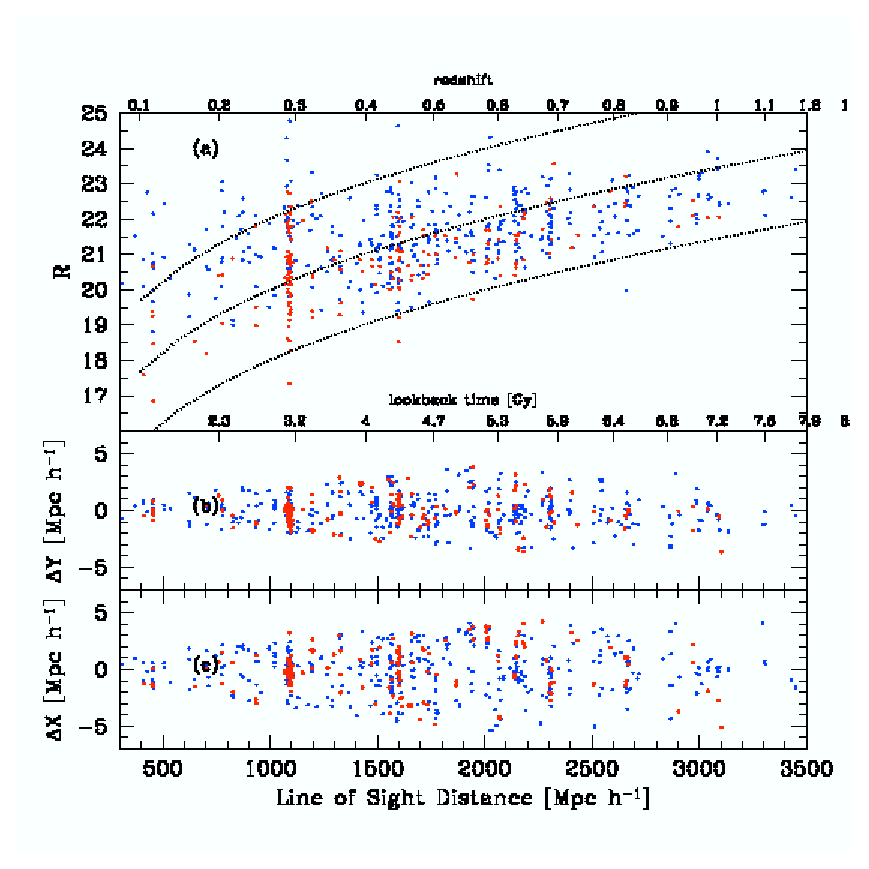
\includegraphics[width=15cm]{figures/egmnFig6.eps}
     \vspace*{-0.0cm}
    \caption{ (a) Magnitude redshift relation for the full sample. The three lines overploted over
the measured points correspond to absolute R magnitudes of -22.5, -20.5, and -18.5.
The distances have been calculated using a cosmology with $\Omega_{0,\Lambda}=0.70$, 
$\Omega_{0,m}=0.30$, $w=-1$, and $\rm H_0 = 75 km~s^{-1}~Mpc^{-1}$ (h = $\rm H_0/75 km~s^{-1}~Mpc^{-1}$). 
Red dots are galaxies with no emission lines and blue dots are galaxies with emission lines.
(b) Cone diagrams in Dec for all the galaxies measured in the field of RX J0054.0-2823. 
The scales is in Mpc calculated using the angular distance for the standard cosmology.
The detection threshold for emission-lines is $\rm EQW([OII])\sim 2-3$\AA. 
(c) Same as (b) but for RA.
}
\label{PieDia}
\end{figure}

\subsection{Indexes}

The 4000~\AA ~ break amplitude and that of 4300~\AA ~ step, which are the main continuum features in the observed wavelength range, 
are given in various tables, together with the [OII] equivalent width.


\subsection{Stellar Population Analysis}
\label{popusynthesis}

In order to study the stellar population quantitatively, we applied a recent version of the spectral population synthesis code, {\it
starlight}\footnote{http://www.starlight.ufsc.br/} \citep{CidFernandes:2004p4742, Gu:2006p5026} to fit the observed and combined spectra. 
The code does a search for the best-fitting linear combination of 45 simple stellar populations
(SSPs), 15 ages, and 3 metallicities ($0.2\,Z_\odot$,
$1\,Z_\odot$, $2.5\,Z_\odot$) provided by \cite{Bruzual:2003p4498} to match
a given observed spectrum $O_\lambda$. The model spectrum
$M_\lambda$ is:
\begin{equation}
M_\lambda(x,M_{\lambda_0},A_V,v_\star,\sigma_\star) =
M_{\lambda_0}
   \left[
   \sum_{j=1}^{N_\star} x_j b_{j,\lambda} r_\lambda
   \right]
   \otimes G(v_\star,\sigma_\star)
\end{equation}
where $b_{j,\lambda} =L_\lambda^{SSP}(t_j,Z_j) / L_{\lambda_0}^{SSP}(t_j,Z_j)$ is the spectrum of the $j^{\rm th}$
SSP normalized at $\lambda_0$, $r_\lambda = 10^{-0.4(A_\lambda - A_{\lambda_0})}$ is the reddening term, $x$ is the
population vector, $M_{\lambda_0}$ is the synthetic flux at the normalization wavelength, and $G(v_\star,\sigma_\star)$ is the
line-of-sight stellar velocity distribution modeled as a Gaussian centered at velocity $v_\star$ and broadened by $\sigma_\star$.
The match between model and observed spectra is calculated as $
\chi^2(x,M_{\lambda_0},A_V,v_\star,\sigma_\star) =
   \sum_{\lambda=1}^{N_\lambda}
   \left[
   \left(O_\lambda - M_\lambda \right) w_\lambda
   \right]^2
$, where the weight spectrum $w_\lambda$ is defined as the inverse
of the noise in $O_\lambda$. For more details we refer to the paper by
\cite{CidFernandes:2005p4910}.

We rebin the 45 SSPs into 5 components according to age: I ($10^6 \leqslant t < 10^8$ yr), II
($10^8 \leqslant t < 5 \times 10^8$ yr), III ($5 \times10^8 \leqslant t < 10^9$ yr),
IV ($10^9 \leqslant t < 2.5 \times 10^{9}$ yr), and V ($t \geqslant 2.5 \times 10^{9}$ yr). 

Here we use {\it starlight} to derive stellar populations models from our spectra in the approximate wavelength range 3000-6000~\AA ~, depending on
$z$. Then we extrapolate the population synthesis spectra to the wavelength range 1000-9000~\AA, in order to fit the
LSST observing window. The Tables in this Note give the stellar fractions obtained in \citep{Giraud:2011}. In the present work we
used a more recent stellar library. Figures 4 to 8 are new.

%SECTION 3

\section{Evolution in the pencil beam}
\label{evolution}

 The redshift range of our pencil beam survey goes up to $z = 1.72$ with a strong decline
above $z \sim 1$. We have truncated the sample at $z = 1.05$.
The spectra of all galaxies in five combined redshift bins are shown in  Figure~\ref{All}, where we show the
absorption systems (top); and emission line galaxies (bottom), separately. \rm 
The S/N ratios of the combined spectra are in the range S/N = 22 - 42, for a 
pixel element of  2.6~\AA. 

% FIGURE 3

\begin{figure}
  \vspace{-0.0cm} 
 \centering
      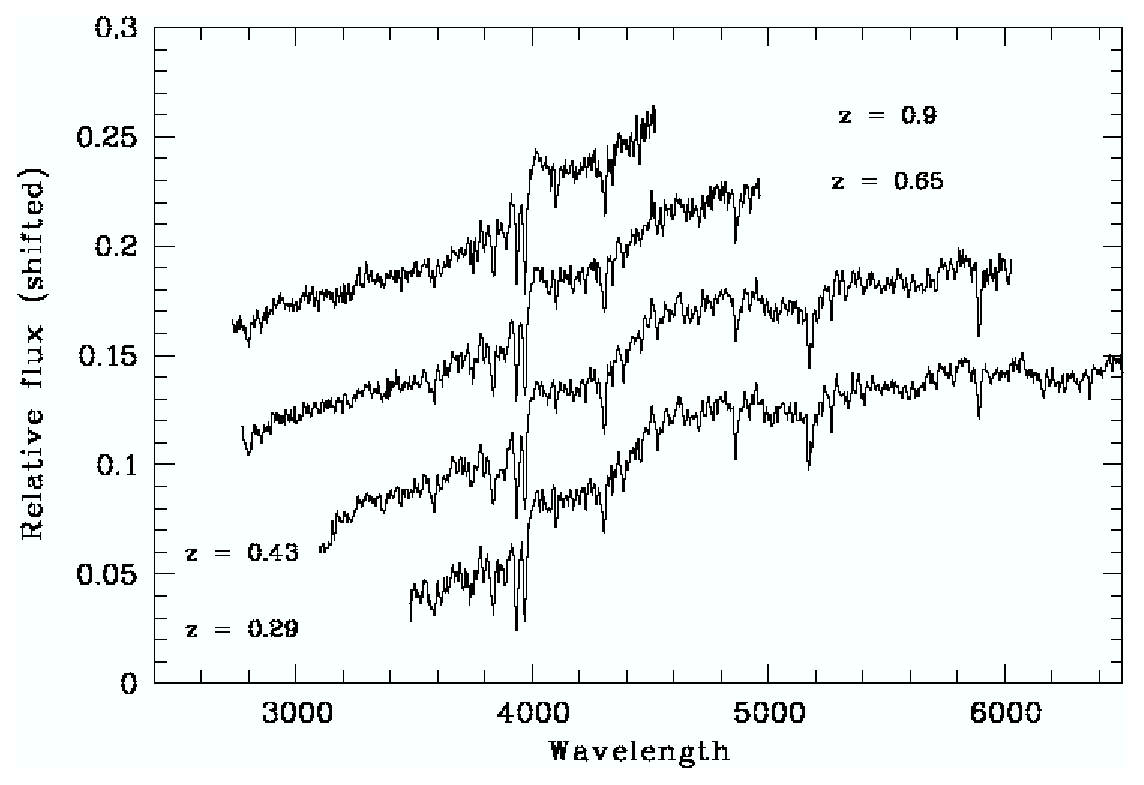
\includegraphics[width=12cm]{figures/egmnFig7b.eps}
      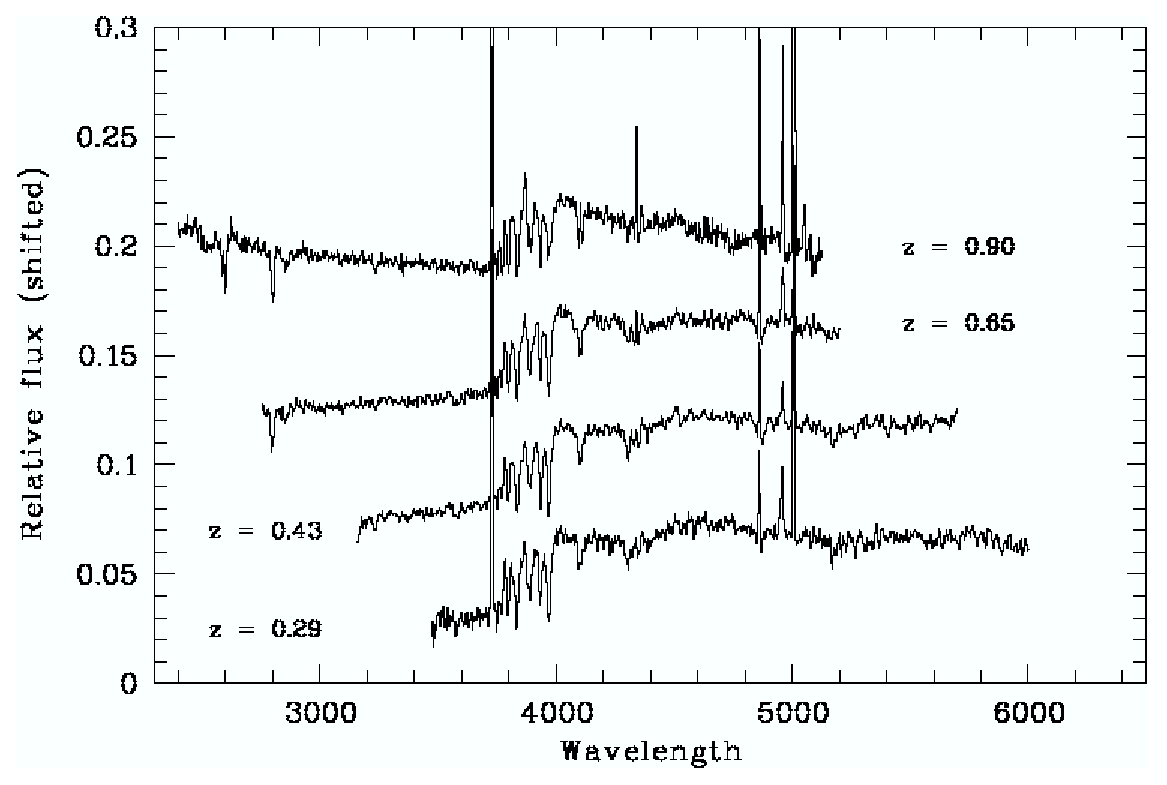
\includegraphics[width=12cm]{figures/egmnFig7c.eps}
  \vspace{-0.0cm}
    \caption{Composite spectra of absorption systems (top); and emission line galaxies (bottom) normalized
		in the wavelength range $\triangle \lambda = 4050 - 4250$~\AA. All individual galaxies are brighter than 
$\rm M_R = -18.8$}
    \label{All}
\end{figure}


The most conspicuous spectral change with redshift is a decrease in flux redward of the G-band from $<z>=0.29$ 
and $<z>=0.43$ to higher $z$ coupled to an increase to the blue of [OII] from  $<z>=0.65$ to  $<z>=0.82$ and higher $z$. Since we 
normalized  the spectra at $\lambda\lambda 4050-4250$\AA, this redistribution of flux
is manifested as a rotation of the continuum around a pivot point at $\lambda\sim 4150$\AA. This rotation of the normalized spectra implies
a systematic change in the galaxy populations entering the sample with redshift: more star forming galaxies at higher $z$,
and more galaxies with old stars at  lower $z$. In order to throw more light 
on this issue, we fitted simple stellar population (SSP) models  to our composite spectra. The  results are summarized in Table~\ref{poptable}.
\rm
% TABLE 2

\begin{table*}
\renewcommand{\arraystretch}{0.9}
\centering 
\caption{  4000\AA\  break amplitudes for the full sample, absorption, and emission galaxies. 
The S/N ratios are those of the combined spectra measured in the wavelength range  4050 - 4250~\AA. The magnitude cutoff is
 $\rm M_R = -18.8$ for all the redshift bins, but is affected by Malmquist bias.}
\begin{tabular}{ c c c c c c c}
      & \multicolumn{2}{c}{Full sample} & \multicolumn{2}{c}{Absorption systems} & \multicolumn{2}{c}{Emission systems} \\
$<z>$ &  D(4000)               & S/N & D(4000)                 & S/N  & D(4000)          & S/N   \\ \hline
& & & & \\
 0.29    & $1.41 \pm 0.04$     & 32  & $1.67 \pm 0.065$          & 23   &  $1.22 \pm 0.02$ & 32       \\
$ 0.43$  & $1.30 \pm 0.03$     & 42  & $1.70 \pm 0.06$        & 22   &  $1.22 \pm 0.01$ & 52      \\
$0.65$   & $1.24 \pm 0.03$     & 38  & $1.60 \pm 0.055$           & 24   &  $1.14 \pm 0.01$ & 35      \\
0.82     & $1.17 \pm 0.04$     & 22  & $1.57 \pm 0.06$      & 18   &  $1.07 \pm 0.02$ & 28      \\     
0.99     & $1.14 \pm 0.04$     & 31  & $1.43 \pm 0.05$         & 23   &  $1.08 \pm 0.02$ & 25      \\
\hline \hline
\label{D4000}
\end{tabular}
\end{table*}

%
% TABLE 3
%

\begin{table*}
\renewcommand{\arraystretch}{0.9}
\centering 
\caption{Stellar population properties of normalized average absorption (abs) and emission (em) spectra in
each redshift bin. The magnitude cutoff is at $\rm M_R = -18.8$, except for the 10 faintest absorption systems at $ z = 0.29$ where
we used all the observed objects.}
\begin{tabular}{ c l c c c c c}
  $<z>$   &  \ \ \ \ \ \ \ \ \ \ log(Age):  &    $<8$  & $8-8.7$ & $8.7-9$ & $9-9.4$& $>9.4$\\ \hline
& & & & & & \\
$0.29$            & abs            	&  0.0\%        & 0.0\%    	&  30.1\%       &  0.1\%  	&  69.8\% \\
         		& abs (10 brightest)    &  0        	& 0      	&  17.4   	&  0    	&  82.4 \\
         		& abs (10 faintest)  	&  0        	& 0      	&  12.0   	&  66.4 	&  21.7 \\
                	& em             	&  16.0    	& 44.1  	&  12.8   	&  1.5  	&  25.7  \\
$0.43$         & abs                   &  0.0          & 0.7           &  11.7         &  6.9          &  80.7 \\
                        & em                    &  28.3         & 14.2          &  16.5         &  36.8         & 4.2  \\
 $0.65$           & abs                   &  0.0          &  0.0          & 18.2          & 38.5          & 43.3 \\
                        & em                    &  33.1         &  0.3          & 65.1          & 1.4           &  0.0  \\
 $0.82$          & abs                   &   0.0         &  0.0          & 86.8          &  3.3          &  9.8\\
                        & em                    &  21.9         & 37.1          & 26.9          & 0.1           & 14.1  \\
 $0.99$          & abs                   &  0.0          & 0.0           & 42.3          & 0.0           & 57.7 \\
                        & em                    &  53.9         & 9.6           & 22.7          & 13.8          & 0.0  \\

\hline \hline
\label{poptable}
\end{tabular}
\end{table*}

%SECTION 4

\section{Absorption line systems}
\label{absorption}


\subsection{Absorption systems as function of redshift}


The normalized and combined spectra of absorption line systems do not show any obvious change in their continuum and their 4000\AA\ break amplitude up to 
$z \approx 0.6$ (Table~\ref{D4000}). There is a small decrease in the  4000\AA\ break at
$z \geq 0.65$ ranging from  $5\%$ at $z \sim 0.65$ to $15 \%$ at $z \sim 1$ while the
$\rm H \delta$ absorption line becomes stronger at $z \geq 0.65$ suggesting 
the presence of increasing numbers of A stars at higher redshifts.  The indexes suggest that these galaxies 
had the bulk of their star formation at $z \geq 1$, while some of the systems at $z > 0.8$ still had clearly 
detectable star formation about 1 Gyr ago.

Our SSP models (Table~\ref{poptable})  indicate that absorption-line systems at $z \geq 0.65$ show more than 
$50 \%$ of stars younger than 2.5 Gyrs, while those at $z \geq 0.8$ had star formation only about one Gyr ago 
(Table~\ref{poptable}).

The extended synthetic spectra from 1000 to 9000 ~\AA ~are similar in the wavelength range  3000 - 9000~\AA~
with however a lower 4300~\AA~ step at high $z$. The models indicate that 80\% of the stellar populations in spectra
of Figure~\ref{Abs-jpg} are older than 1 Gyr except in the spectrum at $z = 1$.

%FIGURE 4

\begin{figure}
  \vspace{-0.0cm} 
 \centering
      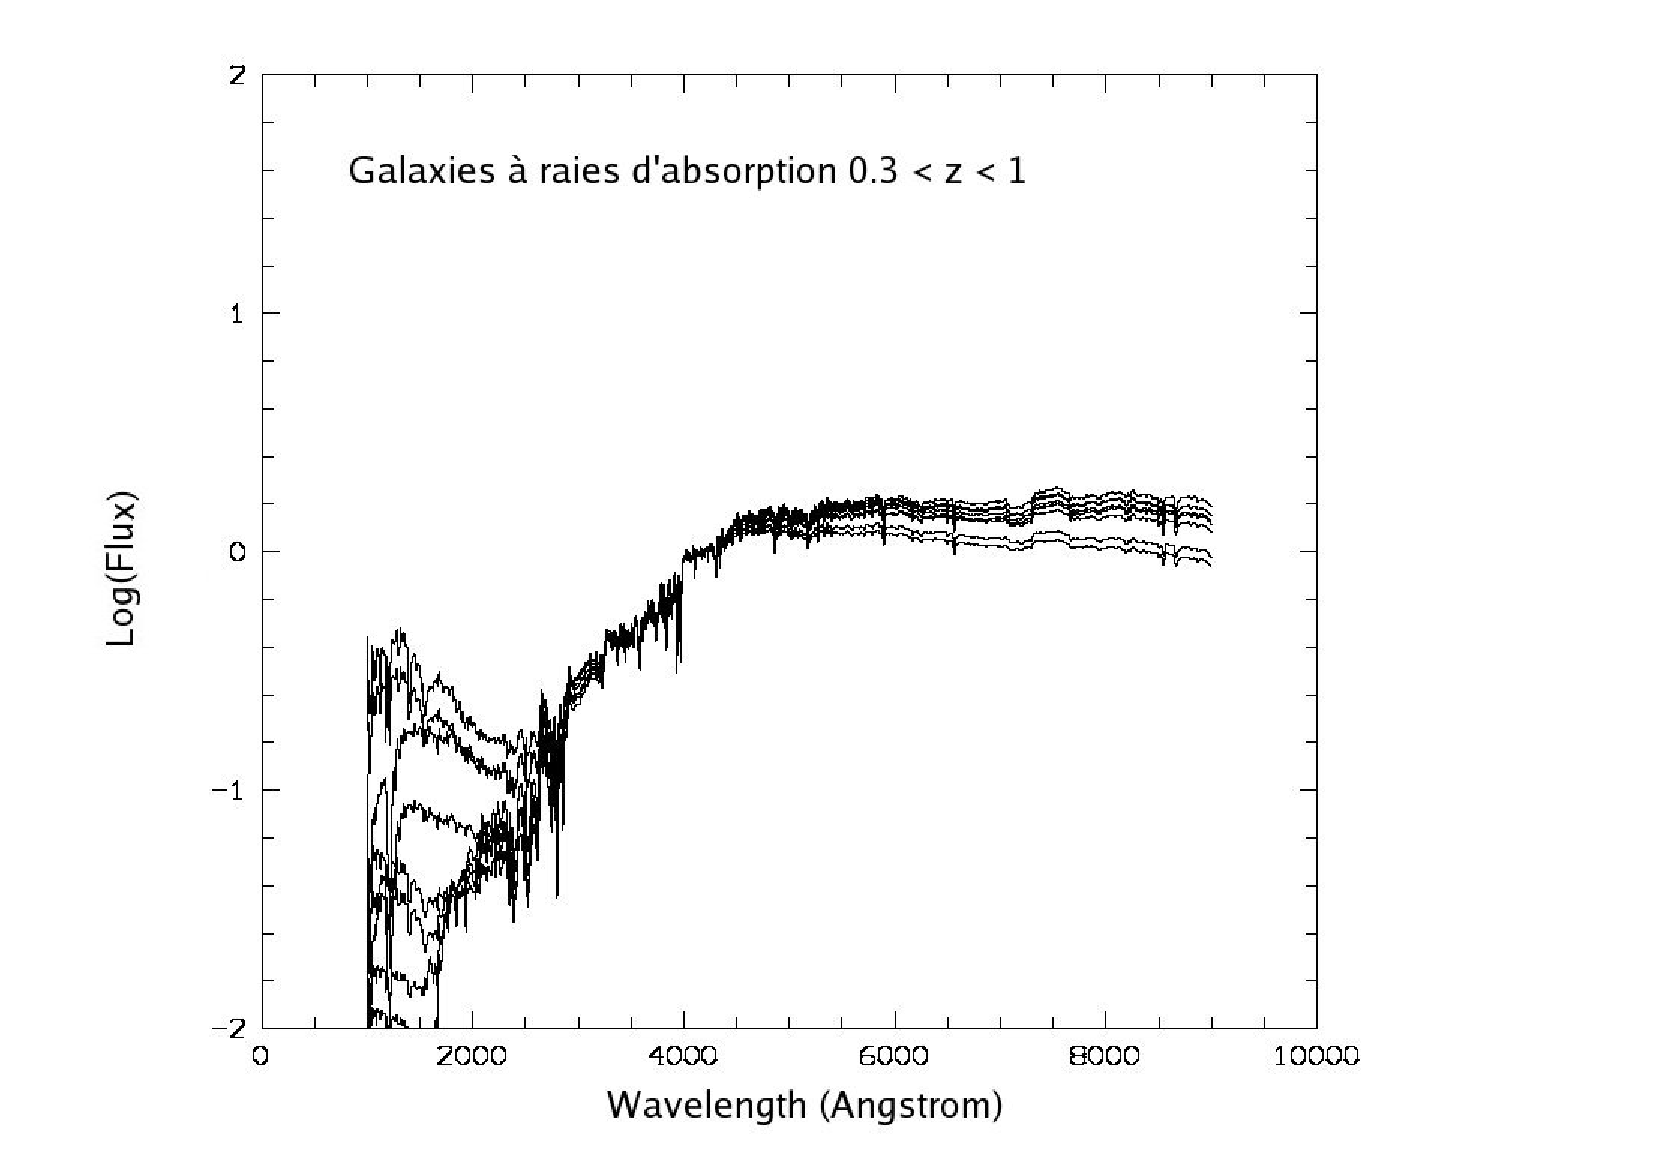
\includegraphics[width=14cm]{figures/Abs.eps}
  \vspace{-0.0cm}
    \caption{Spectral synthesis models of absorption systems derived from galaxies in the range $\rm 0.3 \leq z \leq 1$, normalized in
the wavelength range $\rm 4150-4250\AA$. Flux per \AA~ is in log scale.  }
    \label{Abs-jpg} 
\end{figure}

The UV flux variations in absorption spectra below 3000~ \AA~ depend on the stellar fraction younger than 500 Myr. Our brightest
UV spectra have a tiny fraction ($\leq 2 \%$) of stars younger than 100 Myr, the intermediate ones have a detected
fraction beteen 100 and 500 Myr, while the lowest ones have no detected stars younger than 500 Myr.

The absorption spectrum at $<z> = 0.99$ has 20\% of stars at $\rm 500~ Myr \leq t \leq 1~ Gyr$, so it makes a transition
with post-starbursts galaxies.

\subsection{Post-starbursts}

Post-starbursts E+A galaxies are thought to be in a transition phase between a star-forming period and a 
passively evolving period. Being close to the period of shutdown or quenching of star formation, they probably  
play an important role in the building of early-type systems \citep[e.g.][]{Wild:2009, Yan:2009}.
Past studies of intermediate redshift clusters at $0.3 \leq z \leq 0.6$ have found either a higher fraction of 
post-starbursts in clusters than in the field \citep{Dressler:1999, Tran:2003, Tran:2004p5213}, or a similar fraction \citep{Balogh:1999p4259}.
In fact there is a strong variation in the E+A fraction between the SSDS low redshift survey at $z\sim0.07-0.09$,
and high $z$ surveys at $z \approx 0.5-1$ \citep[VVDS,][]{Wild:2009}, or $z \approx 0.7-0.9$ 
\citep[DEEP2,][]{Yan:2009}.

Synthetic spectra of post-starbursts obtained by fitting selected galaxy spectra
are shown in Figure~\ref{post-starburst}. They all have strong Balmer absorption
lines and have the common property of a large fraction of stars with
age $\rm 200~ Myr \leq t \leq 1~Gyr$. They have similar spectra in the
visible and huge differences in the UV. Nevertheless they seem to form a sequence
which depends on the median age of the burst.

%FIGURE 5

\begin{figure}
   \vspace*{-0.0cm}
   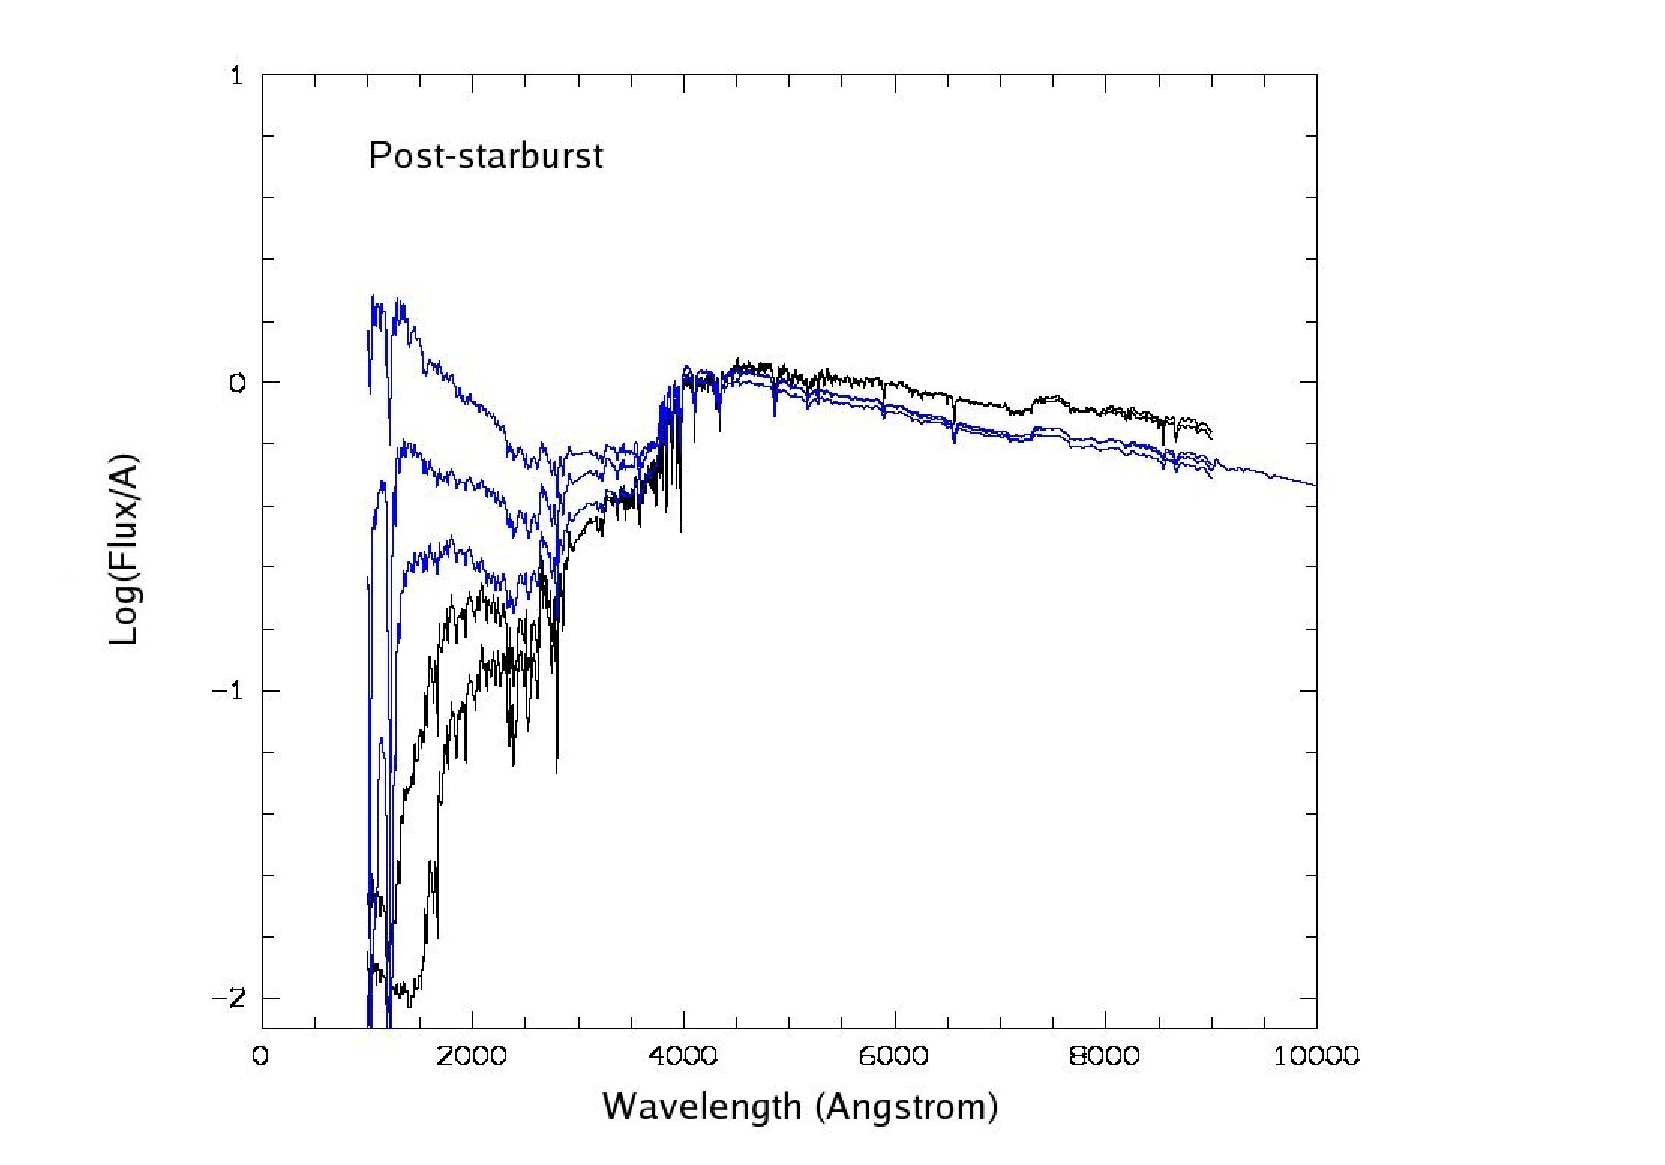
\includegraphics[width=14cm]{figures/post-starburst.eps}
       \vspace*{-0.0cm}
    \caption{Spectral synthesis models of post-starburst galaxies obtained by fitting selected galaxy spectra with Starlight.}
    \label{post-starburst}
\end{figure}

 In the top spectrum coloured in blue, with high UV  in Figure~\ref{post-starburst} the starburst occurred
at a look back time of 200 Myr. The second spectrum coloured in blue has the average colours of 800 K+A galaxies
from the SDSS sample studied by \citep{Melnick:2013}. Melnick
and De Propis used $\rm H\alpha /[NII] $ for the classification. The oldest stars in these spectra are at 6.2 Gyr. In the spectra coloured in 
black the peaks are between 500 and 900 Myrs and
the oldest stars are at 10 Gyr. The
intermediate spectra have peaks at 500 Myrs.

\subsection{Absorption systems as function of luminosity at $z = 0.29$}

The SSP models indicate that on average about 80\% of the stars in the faintest galaxies are younger
than 2.5 Gyr (Table~\ref{poptable}), i.e. were born at $z < 1$. For comparison, 80\% of the stars contributing to the spectrum of the brightest
absorption galaxies in the cluster are older than 2.5 Gyr (Table~\ref{poptable}).

%SECTION 5
  
 \section{Emission-line galaxies}
\label{redsequenceem}

In the visible range the variation of the spectral 
continuum of galaxies with emission lines as function of redshift is significantly stronger than that of
absorption line systems . 

The observed changes in spectral continuum shape in the range $0.3 \leq z \leq 1$, 
in indexes, and in stellar population models take place over cosmological time scales of order 4 Gyr.
Since for single bursts the  models predict such 
variations on time scales \rm of less than 2 Gyr, we  interpret the observed
spectral changes  as an evolutionary sequence
where, on average, galaxies with various bursts at various rates and ages, ``migrate" towards redder types as they evolve.
These results are in agreement with the well known
steep increase in SFR between redshifts 0 and 1 
\citep{Pei:1995p5265, Lilly:1996p4401, Madau:1998p4392, Hopkins:2006p4265}.

\subsection{Partitioning the emission line galaxies in ``red'' and ``blue'' systems by their continuum slope}
\label{parti}

In order to examine the evolution of emission-line galaxies, we partition the sample
in two halves: those with continuum slopes  bluer than the average  and those with continuum 
slopes redder than the average.

To separate the spectra in two halves, we normalize them in the wavelength range
4150\,\AA--4250\,\AA, and then we compare their slopes  in the
range 3600\,\AA--6000\,\AA. The median slope is sample dependant and depends
on evolution but it makes sense since the first group contains
mostly starburst galaxies and the second objects in a more advanced evolutionary stage.
Blue emission lines galaxies have been shown to have higher EQW([OII]) than
the red ones.

\subsection{Blue emission line galaxies}
\label{reservoir}

The average parameters $\rm D(4000)$, $\rm EQW([OII])$,
and  $\rm EQW(H\delta)$ of the spectra obtained by combining the blue half of emission systems
 are given in Table~\ref{blueEQW}.

% TABLE 4

\begin{table*}
\renewcommand{\arraystretch}{0.9}
\centering 
\caption{D(4000) and equivalent widths of  [OII] and  H$\delta$  of  average ``blue'' emission-line galaxies. Values marked (*) have  H$\delta$ both in absorption and in emission.\rm}
\begin{tabular}{ l c c c c} 
  $<z>$   & $\rm D(4000)$     & $\rm EQW([OII])$ &  $\rm EQW(H\delta)$ &  S/N  \\ \hline
& & & & \\
 0.29     & $ 1.11 \pm 0.01$  &  $34.3 \pm 0.5$  &   $-4 \pm 0.5$  (*) &  23   \\
0.43  & $ 1.12 \pm 0.01$  & $27.9 \pm 0.4$   & $-2.84 \pm 0.08$    &  49 \\
0.65  & $ 1.09 \pm 0.01$  & $30.3 \pm 0.7$   & $-5 \pm 0.5$  (*)   &  28 \\
 0.82     & $ 1.04 \pm 0.02$  & $53.1 \pm 0.8$ & $-6 \pm 0.5$ (*)      &  18 \\
0.9   & $ 1.02 \pm 0.015$ & $53.8 \pm 0.8$ & $-5.5 \pm 0.5$  (*)   &  23 \\ 
0.99      & $ 1.02 \pm 0.02$  & $58.8 \pm 0.9$ & $-5 \pm 0.5$   (*)    &  12 \\
\hline \hline
\label{blueEQW}
\end{tabular}
\end{table*}


% FIGURE 6

%\begin{figure}
  %\centering
  %\vspace{-0.0cm}
     % 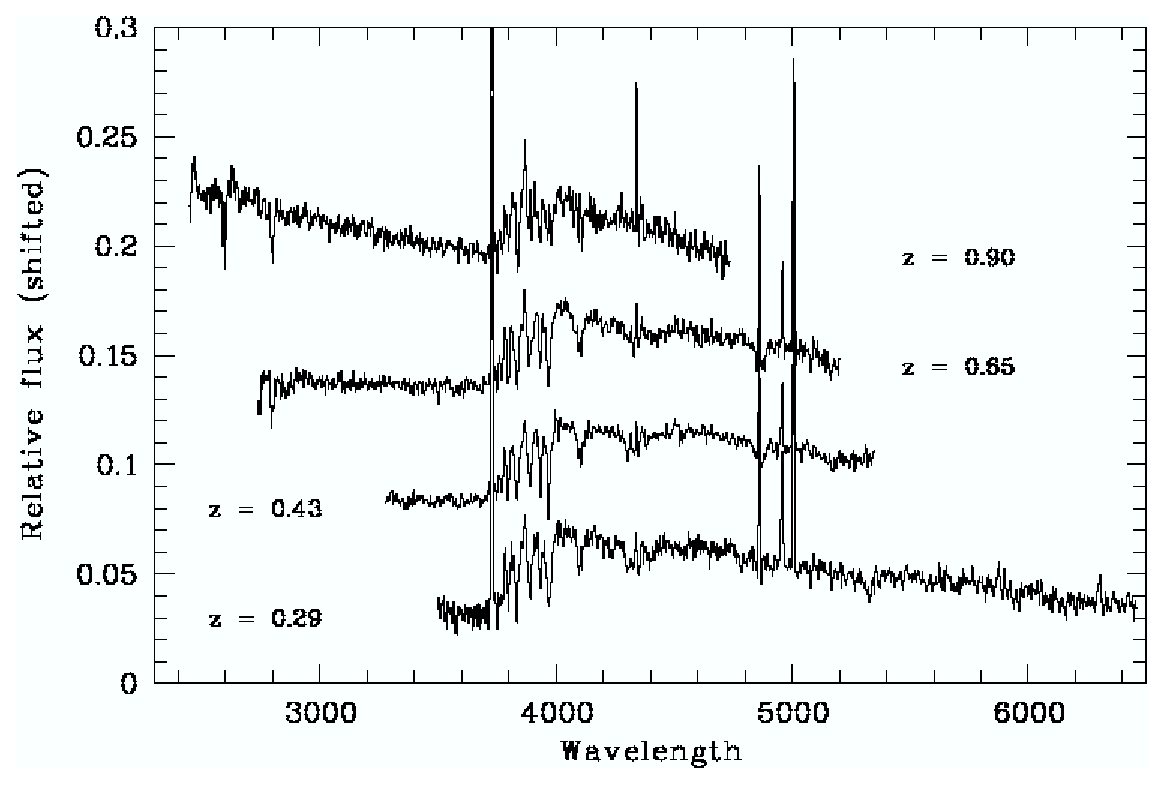
\includegraphics[width=11cm]{figures/egmnFig12a.eps}
      %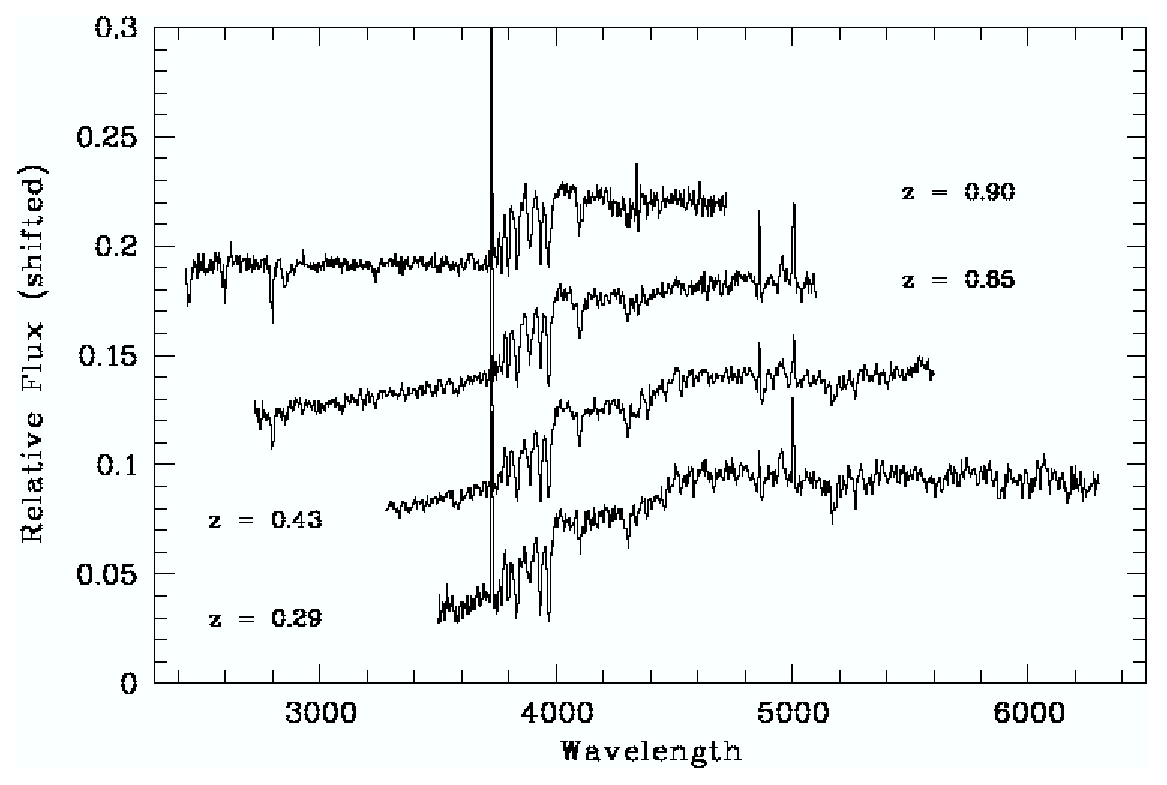
\includegraphics[width=11cm]{figures/egmnFig12b.eps}
    %\vspace{0.0cm}
    %\caption{Composite spectra of galaxies with emission lines: (top) blue half; (bottom) red half.
%		Spectra have been normalized in the wavelength range $\triangle \lambda = 4050 - 4250$~\AA\ and shifted
%		for clarity.}
  %   \label{emgal}
%\end{figure}


% FIGURE 6

\begin{figure}
  \centering
  \vspace{-0.0cm}
  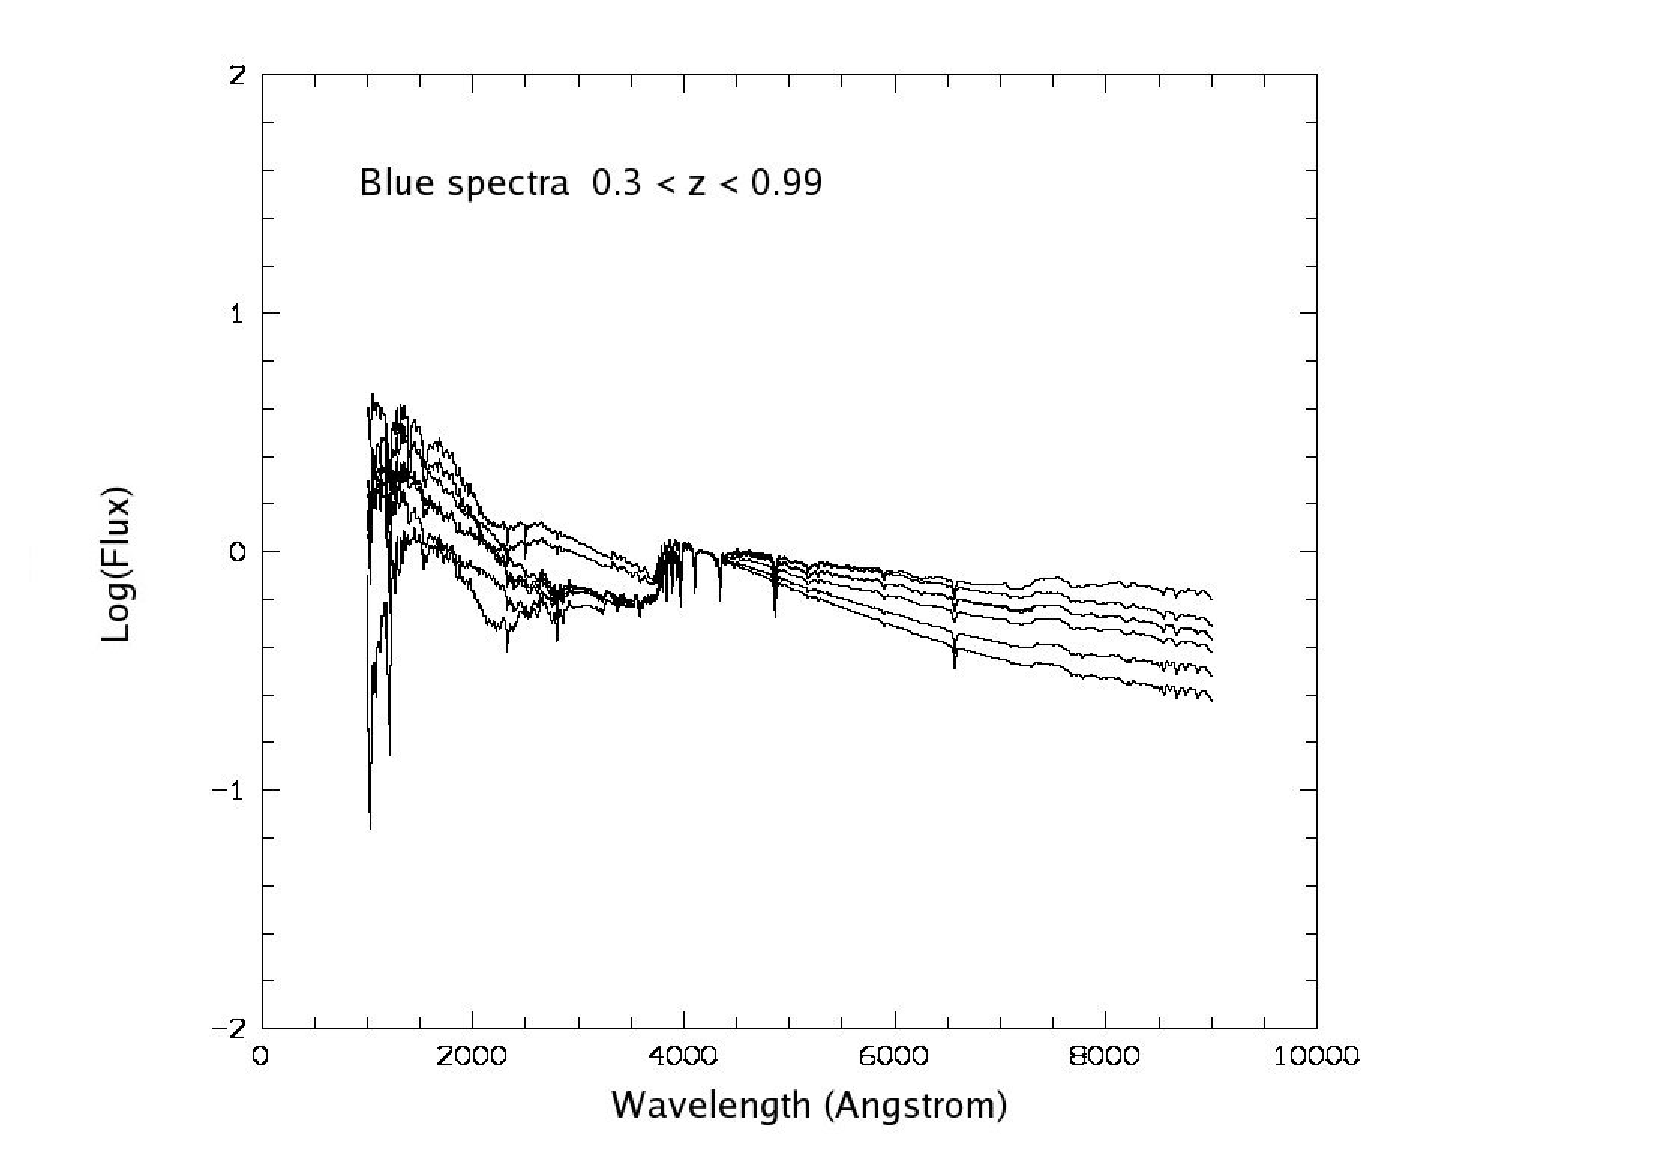
\includegraphics[width=14cm]{figures/Em-blue.eps}
 \vspace{0.0cm}
    \caption{Spectral synthesis models obtained by fitting spectra of blue emission lines galaxies}
     \label{Emblue-jpg}
\end{figure}



\subsection{Red emission-line galaxies}
\label{tracks} 

% FIGURE 7

\begin{figure}
  \centering
  \vspace{0.0cm}
  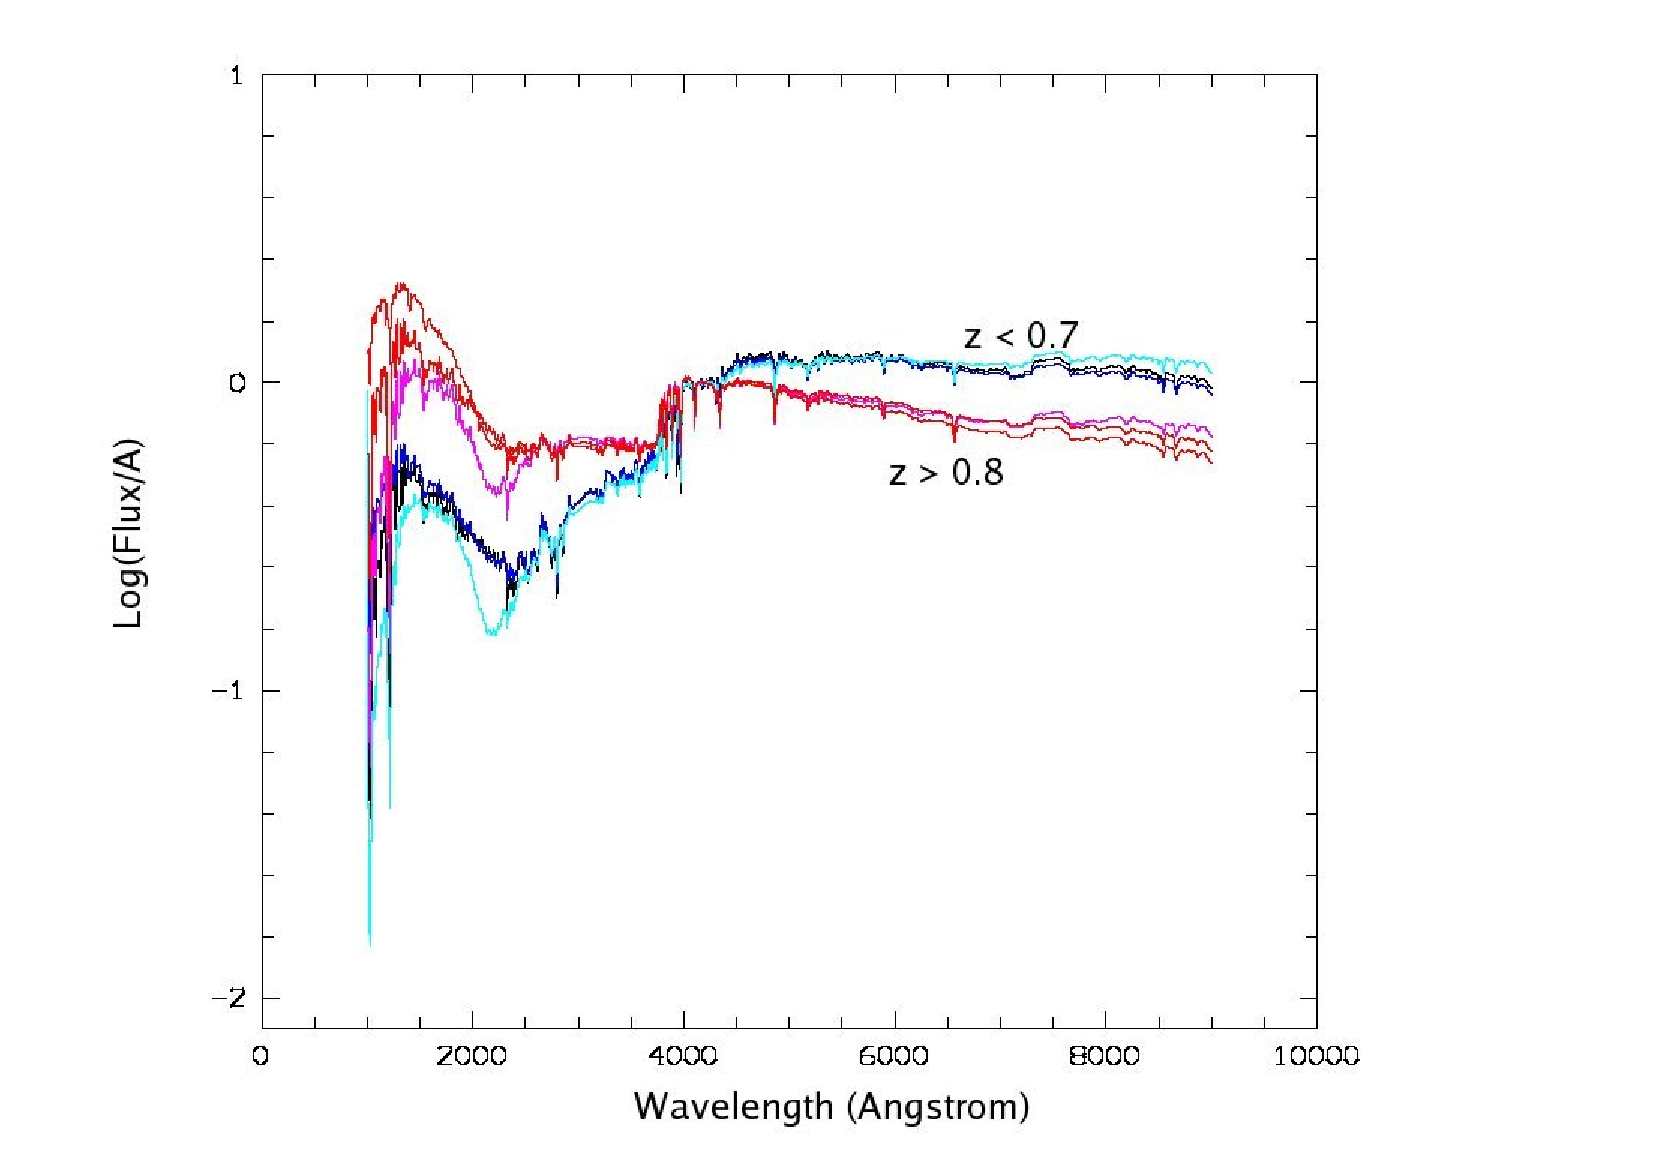
\includegraphics[width=14cm]{figures/Em-red.eps}
 \vspace{0.0cm}
    \caption{Spectral synthesis models obtained by fitting spectra of red emission lines galaxies}
     \label{Emred-jpg}
\end{figure}

After having isolated the two extremes of our galaxy population: starburst dominated emission-line galaxies, and absorption-line systems, 
we now turn to the galaxies in intermediate evolutionary stages. 
The most conspicuous changes in the spectra are the systematic increase in UV continuum and [OII] strength with redshift \rm

In order to quantify the evolution of the continuum to the red of the G band, we introduce a G-step index as the ratio of the $[4550 - 4650]$~\AA\ to the  $[4150 - 4250]$~\AA\ fluxes. The resulting values are given in Table~\ref{GD}. There is an increase of $16 \%$ in the G-step
index between $<z>=0.65$ and $<z>=0.29$ and a corresponding increase of $9 \%$ in the D(4000) break.
These variations reach respectively $26 \%$ and $15 \%$ over the redshift range $<z> = 0.9$ to  $<z>=0.29$.
The G-step  of absorption systems, also given in  Table~\ref{GD} for comparison, is in all cases
larger than the values for the red emission-line galaxies
 
% TABLE 5

\begin{table*}
\renewcommand{\arraystretch}{0.9}
\centering 
\caption{ Equivalent widths of [OII] and $\rm H\delta$ in absorption,
4000\AA\ break amplitudes, and  G-step indexes for  ``red'' emission systems.
 The number of galaxies in each bin ($N_{gal}$) is given in the second column
and the dispersions   in EQW([OII]) and  D(4000) within each bin are given in
parenthesis.
The values of $\rm EQW(H\delta)$ marked with a (*) are measured as in
Table~\ref{blueEQW}. 
 The G-steps of absorption systems are listed in the last column for comparison.\rm }

\begin{tabular}{ l c c c c c c c}
$<z>$ 	&   $N_{gal}$ & $\rm EQW([OII])$  &  D(4000)           & $\rm EQW(H\delta)$ &    G step                                & S/N  &   G step (abs)   \\ \hline
& & & & & & & \\
0.29  	&   13 	& $13.2 \pm 0.3$  (11)   	& $1.324 \pm 0.038$  (0.53)  & $-1.89 \pm 0.05$   & $1.221 \pm 0.012$          &  27   & $1.470 \pm 0.018$   \\
0.43         &  38  	& $10.7 \pm 0.5$  (4.6)   	& $1.317 \pm 0.038$  (0.15) & $-2.32 \pm 0.05$   & $1.164 \pm 0.012$   &  34   & $1.423 \pm 0.018$   \\
0.65         & 29 		& $14.3 \pm 0.5$  (6.0)  	& $1.197 \pm 0.037$  (0.10) & $-4.42 \pm 0.05$   & $1.054 \pm 0.010$   &  37   & $1.369 \pm 0.017$   \\
0.82  	&   11 	& $26.7 \pm 0.7$  (12.5)  	& $1.118 \pm 0.038$  (0.08) &  $-4.6 \pm 0.5$ (*)  & $0.977 \pm 0.019$         &  22   &        -            \\
0.9 	        &  23 	    & $29.5 \pm 0.6$  (19)   	& $1.132 \pm 0.040$  (0.09)  & $-5.3 \pm 0.3$ (*)  & $0.971 \pm 0.015$ &  25   & $1.325 \pm 0.034$   \\
0.99  	&   9 		&$30.3 \pm 0.7$  (19.7)   	& $1.150 \pm 0.050$  (0.07) &  $-5.5 \pm 0.5$ (*)  & $0.965 \pm 0.020$ &  20   &        -           \\

\hline \hline
\label{GD}
\end{tabular}
\end{table*}

 The SSPs clearly 
show that star formation in red emission-line galaxies is fading at $z < 0.5$.
Extrapoltaing the SSP fits from $\rm 1000~\AA$ to $\rm 9000 ~\AA$ clealy shows the decline of the $4300~\AA$ step and the increase of
UV flux with z or increasing look-back time (Figure~\ref{Emred-jpg}). There are large variations in the UV around these median
spectra.

% TABLE 6
 
\begin{table*}
   \renewcommand{\arraystretch}{0.9}
   \centering 
   \caption{Stellar population properties of red emission-line galaxies}
   \begin{tabular}{ l c c c c c c }
          $<z>$            & \multicolumn{5}{c}{log Age} &$\rm \chi^2$ \\ \hline
&  $<8$  & $8-8.7$ & $8.7-9$ & $9-9.4$ & $>9.4$   &  \\ \hline
& & & & & & \\
              
$0.29$            &    0.0 &   28.3 &          16.6  &        25.5  &         29.5  & 1.20                \\
$0.43$       &     9.0 &   20.8   &       30.8  &        32.7 &          6.7   & 0.70                \\
$0.65$        &    13.8 &   25.1   &       40.9  &        20.2 &          0.0   & 0.68                 \\
$0.9$         &    18.0 &   33.2   &       15.2  &        33.6  &         0.0   & 0.75                  \\
   \hline \hline
   \label{redpop}
   \end{tabular}
\end{table*}

%SECTION 6

\section{Two main classes of spectra?}

%FIGURE 8

\begin{figure}
  \centering
  \vspace{0.0cm}
  \includegraphics[width=14cm]{figures/UVspectra.eps}
 \vspace{0.0cm}
    \caption{Continuum spectra divided in two classes by their relative peak amplitude in the UV.}
     \label{2classes}
\end{figure}


The main difference in flux spectra measured in normalized SEDs is in the UV where amplitude changes by
$\rm \sim 2.5dex$ between low and high relative UV fluxes below 2000 \AA. Graphically, 
there are two main classes of spectra: those with low or high UV which are shown in Figure~\ref{2classes}.
It may be strange to classify galaxy spectra by the existence of recent bursts that cover short episodes of galaxy
lifes, but one may argue that this is not more than recovering the two main classes of stars. Moreover this
distinction in two classes may be efficient in a photo-z approach: red spectra, which have no (or weak) UV bump,
are those in which the the 4000 \AA~ break is the largest, namely the easiest to detect, while those with a UV bump have
a low 4000 \AA~ break amplitude AND a UV bump. In red spectra a photo-z code will search for a step,
in blue spectra that will be for a valley. Intermediate spectra will have a detected UV bump and still a quite large break
amplitude. This simple approach will be efficient as soon as the peak at 1500 \AA~ enters a ground based UV filter 
centered at 3500 \AA, that is by $z = 1$, and should cover the ``spectroscopic desert" between $z = 1.2$ and $z = 2$.
At low $z$,  $g - i$ colour should be discriminant as well.

The red part of our absorption spectra is flatter than that of Gorecki et al's (2104) templates, in
particular at larger wavelengths than the 4300 \AA ~ step. Our mixing should include
more old stars and a different intermediate-to-old age ratio. A similar difference may occur
for red spirals at $ z \leq 0.6-0.7$. Our blue emission lines form a sequence between Gorecki et
 al's \#3 to \#5 spectra.  Our post-starburts are also well described by Gorecki et al's red spectra.

%SECTION 7

\section{Summary}
\label{conclusion}

We have considered a sample of galaxies spectra in a pencil beam survey at $z \leq 1$ to derive the main
features of spectra including those that may change with $z$.

The 4000 \AA~break is the only feature in all spectra at all redshifts. 

There are two distinct classes of
spectra depending on the spectral slope above 3000  \AA ~: 1) Early absorption systems,  most
of the post-starbursts, red spirals at $z \leq 0.6-0.7$ 2) Blue starforming galaxies and recent
post-starbursts. Among the first class the 4300 \AA~ step declines with $z$ at about
$z = 0.6-0.7$ for red spirals, and at about $z = 1$ for ellipticals.

All spectra with some recent stellar activity shows a clear UV excess between 1500 \AA~ and 2500 \AA.

Large variations in the UV  due to a residual fraction of young stars in early absorption
systems or to the age and intensity of the most recent starburst in post-starburst galaxies
may occur at any look back time.

Red emission lines galaxies show an increasing fraction of young stars with $z$ and a decreasing
fraction of stars older than $\rm \leq 2.5~ Gyr$.

In each redshift bin early absorption systems are brighter than red spirals, which in turn are brighter than 
blue star-forming objects. Starbursts were brighter at large look back time than at low $z$ (Table 1).
 
\begin{acknowledgements}

\end{acknowledgements}

\begin{thebibliography}{}

%\bibitem[Adelman-McCarthy et al 2006]{Adelman:2006} Adelman-McCarthy, J.K., et al, 2006, ApJS 162, 38


\bibitem[Balogh et al. 1999]{Balogh:1999p4259} Balogh, M. L., Morris, S. L., Yee, H. K. C., Carlberg, R. G., \& Ellingson, E., 1999, ApJ 527, 54   


%\bibitem[Baugh et al. 1996]{Baugh:1996p5586} Baugh, C.M.,Cole, S., \& Frenk, C.S., 1996, MNRAS.283, 1361


\bibitem[Bell et al. 2004]{Bell:2004p4427} Bell, E. F., et al, 2004, ApJ 608, 752

\bibitem[Bell et al. 2005]{Bell:2005p4431} Bell, E. F., et al, 2005, ApJ 625, 23


%\bibitem[Blake et al. 2004]{Blake:2004} Blake, C., et al., 2004, MNRAS 355, 713


\bibitem[Blanton et al. 2003]{Blanton:2003p4432} Blanton, M. R., et al, 2003, ApJ 594, 186


%\bibitem[Bundy et al  2009]{Bundy:2009} Bundy, K., et al.,  2009, astro-ph 0912.1077v1

%\bibitem[Bundy et al 2008]{Bundy:2008} Bundy, K., et al., 2008, ApJ 681, 931


\bibitem[Bruzual \&  Charlot 2003]{Bruzual:2003p4498}  Bruzual G., \&  Charlot S., 2003, MNRAS, 344, 1000

\bibitem[Cassata et al. 2007]{Cassata:2007p4503} Cassata, P., et al, 2007, ApJS 172, 270

\bibitem[Cid Fernandes et al. 2004]{CidFernandes:2004p4742} Cid Fernandes R. , et al., 2004, MNRAS, 355, 273

\bibitem[Cid Fernandes et al. 2005]{CidFernandes:2005p4910} Cid Fernandes R., Mateus A., Sodre L., Stasinska G.,
Gomes J., 2005, MNRAS 358, 363
 
\bibitem[Clemens et al. 2006]{Clemens:2006p5321} Clemens, M.S., Bressan, A., Nikolic, B., Alexander, P., \& Rampazzo, R., 2006, MNRAS 370, 702


%\bibitem[Cooper et al. 2006]{Cooper:2006p4926} Cooper, M. C. et al, 2006, MNRAS 370, 198


\bibitem[Cowie et al. 1996]{Cowie:1996p4930} Cowie, L. L., Songaila, A., Hue, E. M., \& Cohen J. G., 1996,  AJ 112, 839

\bibitem[Cucciati et al. 2006]{Cucciati:2006p4973} Cucciati, O., et al (the VVDS Team), 2006, A\&A 458, 39

\bibitem[Dickinson et al. 2003]{Dickinson:2003p4993} Dickinson, M., Papovich, C., Fergusson, H.C., Budavari, T., 2003, ApJ 587, 25

\bibitem[Dressler et al. 1999]{Dressler:1999} Dressler, A., et al., 1999, ApJS 122, 51

\bibitem[Faber et al. 2007]{Faber:2007} Faber, S. et al, 2007, ApJ 665, 265

\bibitem[FORS1+2 Manual (2005)]{fors:2005} FORS1+2 User Manual VLT-MAN-ESO-13100-1543 Issue 4, 2005

\bibitem[Franzetti et al. 2007]{Franzetti:2007p4273} Franzetti, P., et al (the VVDS Team), 2007, A\&A 465, 711


%\bibitem[Garilli et al. 2008]{Garilli:2008p5000} Garilli, B., et al (the VVDS Team), 2008, astro-ph 0804.4568


\bibitem[Giallongo et al. 2005]{Giallongo:2005p5002} Giallongo, E., et al, 2005, ApJ 622, 116

%\bibitem[Goto 2007]{Goto:2007} Goto, T., 2007, MNRAS 377, 1222



%\bibitem[Granato et al. 2004]{Granato:2004} Granato, G.L., et al., 2004, ApJ 600, 580

\bibitem[Giraud et al. 2011]{Giraud:2011} Giraud, E. et al., 2011 RAA 11, 245

\bibitem[CDS Catalog; Giraud et al. 2012]{Catalog:2012} Giraud, E. et al.,  CDS Catalog 2012, 2012yCatp040001104G

\bibitem[Gorecki et al. 2014]{Gorecki:2014} Gorecki, A. et al,. 2014,  A\&A 561, 128	

\bibitem[Gu et al. 2006]{Gu:2006p5026} Gu Q. et al.  2006, MNRAS, 366, 480
 
%\bibitem[Hamilton 1985]{Hamilton:1985} Hamilton, D., 1985 ApJ, 297, 371

\bibitem[Hammer et al. 2005]{Hammer:2005p5042} Hammer, F., et al, 2005, A\&A 430, 115



\bibitem[Hogg et al. 2002]{Hogg:2002p5043} Hogg, D. W., et al, 2002, AJ 124, 646


\bibitem[Hopkins \& Beacom 2006]{Hopkins:2006p4265} Hopkins, A. M., \& Beacom, J. F., 2006, ApJ 651, 142


\bibitem[Kodama et al. 2004]{Kodama:2004p5056} Kodama, T., et al, 2004, MNRAS 350, 1005

\bibitem[Koyama et al. 2007]{Koyama:2007p5060} Koyama, Y., Kodama, T., Tanaka, M, Shimasaku, K., \& Okamura, S., 2007, MNRAS 382, 1719
 
\bibitem[Le F\`evre et al. 2007]{LeFevre:2007p5105} Le F\`evre, O. et al, 2007, ASPC 379, 138

\bibitem[Lilly et al. 1996]{Lilly:1996p4401} Lilly, S. J., Le Fevre, O., Hammer, F., \& Crampton, D., 1996, ApJ 460, L1


%\bibitem[Lin et al. 2008]{Lin:2008} Lin, L., et al., 2008, ApJ 681, 232


\bibitem[Madau et al. 1998]{Madau:1998p4392} Madau, P., Pozzeitti, L., \& Dickinson, M., 1996, ApJ 498, 106

\bibitem[Melnick \& De Propis 2013]{Melnick:2013} Melnick, J., \& De Propis,  R. 2013, MNRAS 431, 2034	

\bibitem[Pei \& Fall 1995]{Pei:1995p5265} Pei, Y. C., \& Fall, S. M., 1995, ApJ 454, 69

\bibitem[Renzini 2006]{Renzini:2006p5117} Renzini, A., 2006, ARA\&A 44, 141

\bibitem[Renzini 2007]{Renzini:2007p5120} Renzini, A., 2007, ASPC 390, 309


%\bibitem[Sarzi et al. 2006]{Sarzi:2006} Sarzi, M., et al., 2006, MNRAS 366, 1151

%\bibitem[Scarlata et al. 2007]{Scarlata:2007} Scarlata, C., et al., 2007, ApJS 172, 406 


\bibitem[Scoville et al. 2007a]{Scoville:2007p5138} Scoville, N., et al, 2007a, ApJS 172, 1

\bibitem[Scoville et al. 2007b]{Scoville:2007p5137} Scoville, N., et al, 2007b, ApJS 172, 150




\bibitem[Strateva et al. 2001]{Strateva:2001p5121} Strateva, I., et al, 2001, AJ 122, 1861


%\bibitem[Tanaka et al. 2005]{Tanaka:2005p5158} Tanaka, M., et al, 2005, MNRAS 362, 268


\bibitem[Thomas et al. 2005]{Thomas:2005p5302} Thomas, D., Maraston, C., Bender, R., \& Mendes de Oliveira, C., 2005, ApJ 621, 673


\bibitem[Tran et al. 2007]{Tran:2007p5181} Tran, K.-V. H., et al, 2007, ApJ 661, 750

\bibitem[Tran et al. 2004]{Tran:2004p5213} Tran, K.-V. H., et al, 2004, ApJ 609, 683

\bibitem[Tran et al. 2003]{Tran:2003} Tran, K.-V. H,. et al, 2003, ApJ 599, 865



\bibitem[Weiner et al. 2005]{Weiner:2005} Weiner, B.J., et al, 2005, ApJ 620,  595

\bibitem[Wild et al. 2009]{Wild:2009} Wild, V., et al, 2009, MNRAS 395, 144

\bibitem[Yan et al. 2009]{Yan:2009} Yan, R., et al, 2009, MNRAS 398, 735

\bibitem[York et al. 2000]{York:2000p5225} York, D. G., et al, 2000, AJ 120, 1579


\end{thebibliography}

%\bibliography{zbiblio} % your references Yourfile.bib
\end{document}
 
